\subsection{Back-Propagation}
\label{sec:back-propagation}

Often mistaken for the whole learning algorithm, 
back-propagation just refers to the algorithm for computing the gradient of a computational graph.
It is called back-propagation because we evaluate the gradient for the output layer backwards to the input layer.
In some way it can be understood as a counter part to the forward propagation.
As already discussed, forward propagation describes the process of calculating the output \(\hat{\fat{y}}\) of a feedforward network for a given input \(\fat{x}\).
Back-propagation on the other hand now works it way from the output layer to the input layer in order to compute the gradient for a given input \(\fat{x}\), a calculated output \(\hat{\fat{y}}\) and
a \enquote{wanted} output \(\fat{y}\).

A common misbelief, is that the back-propagation is performed on the feedforward network itself, whereas it is rather done on the computational graph of the cost function.
Optimizing the \emph{weights} in the graph of the cost function also optimizes them in the network!
Since the back-propagation only computes the gradient, the \enquote{real} learning is performed by an \emph{optimizing} algorithm, such as \emph{stochastic gradient descent} \fref{sec:stochastic-gradient-descent}.

\paragraph{Chain Rule of Calculus.}
The chain rule of calculus describes how to calculate the derivative of a function that is composed of other functions.
Let \(f: \mathbb{R} \rightarrow \mathbb{R}\) and \(g: \mathbb{R} \rightarrow \mathbb{R}\) both be differentiable.
If \(y = g(x)\) and \(z = f(y) = f(g(x))\), then
\begin{equation}
    \frac{\partial z}{\partial x} = \frac{\partial z}{\partial y} \frac{\partial y}{\partial x}.
\end{equation}
This can of course also be written as
\begin{equation}
    (f(g(x)))^\prime = f^\prime (g(x)) g^\prime(x).
\end{equation}
This can now be extended to arbitrary dimension.
Let \(g: \mathbb{R}^m \rightarrow \mathbb{R}^n\) and \(f: \mathbb{R}^n \rightarrow \mathbb{R}\).
If \(\fat{y} = g(\fat{x})\) and \(z = f(g(\fat{x})) = f(\fat{y})\), then
\begin{equation}
    \frac{\partial z}{\partial \fat{x}_{i}} = \sum_{j} \frac{\partial z}{\partial \fat{y}_{j}} \frac{\partial \fat{y}_{j}}{\partial \fat{x}_{i}}.
\end{equation}
Using the \(\nabla\) operator for the gradient, this can also be written as
\begin{equation}
    \label{eq:jacobian-vector-product}
    \nabla_{\fat{x}} z = \bigg( \frac{\partial \fat{y}}{\partial \fat{x}} \bigg)^{T} \nabla_{\fat{y}} z,
\end{equation}
where \(\frac{\partial \fat{y}}{\partial \fat{x}}\) is the \(n \times m\) Jacobian of \(g\).
Since feedforward networks often work with tensors of arbitrary dimension and not vectors, we would have to change our notation a bit in order to deal with them.
We would simply \enquote{flatten} the tensor and use multiple coordinates as indices for the dimensions.
However I am not going to introduce this here, since the concept can already be understood with vectors. \\

The general idea of the back-propagation algorithm is simple.
If we want to compute the gradient of \(z\) with respect to \(x\) we start at the node \(z\).
We observe that the gradient of \(z\) with respect to \(z\) is \(1\), since \(\frac{\partial z}{\partial z} = 1\).
We then compute the gradient with respect to each parent of \(z\) by multiplying the current gradient by the Jacobian that produced \(z\).
This means we propagate backwards through the network by multiplying with Jacobians until we reach \(x\).
If there are multiple paths, we simply take them each after another.

More formally this means that each node in the computational graph corresponds to a variable (in our case a vector).
Each variable \(\fat{v}\) has now the following subroutines:
\begin{itemize}
    \item \texttt{operation(\(\fat{v}\))}, gets the mathematical operation that defines \(\fat{v}\),
    which is represented by the edges flowing into \(\fat{v}\) and the relation, e.g. matrix multiplication
    \item \texttt{children(\(\fat{v}\))}, returns an array that contains the variables that are children of \(\fat{v}\) in the graph
    \item \texttt{parents(\(\fat{v}\))}, returns an array that contains the variables that are parents of \(\fat{v}\) in the graph 
\end{itemize}
Furthermore every operation \texttt{op} is associated with a \texttt{back\_prop} operation, that computes the product described by \fref{eq:jacobian-vector-product}.
Let \(\fat{C} = \fat{AB}\), and the gradient of a scalar \(z\) with respect to \(\fat{C}\) be \(\fat{g} \in \mathbb{R}^n\).
Then \texttt{back\_prop} has to define the gradient of matrix multiplication for \(\fat{A}\) and \(\fat{B}\).
This means that \texttt{op.back\_prop(parents(..), \(\fat{A}\), \(\fat{g}\))} evaluates to \(\fat{g}\fat{B}^T \in \mathbb{R}^n\), because \(\frac{\partial \fat{C}}{\partial \fat{A}} = \fat{B}^T\).
Analogously, the call of \texttt{op.back\_prop(parents(..), \(\fat{B}\), \(\fat{g}\))} evaluates to \(\fat{A}^T\fat{g} \in \mathbb{R}^n\).
Formally the call of \texttt{op.back\_prop(parents(..), \(\fat{V}\), \(\fat{g}\))} returns
\begin{equation}
    \sum_{i} \big( \nabla_{\fat{V}} \texttt{op.f(parents(..))}_{i} \fat{G}_{i} \big),
\end{equation}
where \texttt{op.f} is the mathematical relation (e.g. matrix multiplication).
The two dots in the call of the \texttt{parent(..)} function refer to the current node we are at.
It is of great importance that \texttt{op.back\_prop} always pretends that all of its inputs are distinct.
Take for example the function \(x^2\) the \texttt{back\_prop} should now for both inputs return \(x\).
It will later add those two \(x\) together to receive the correct derivate of \(2x\).

By making use of the \texttt{back\_prop} function like this, we receive a very general back-propagation algorithm. \\

\paragraph{Back-Propagation example.}
With the Back-propagation we can determine the gradient of \fref{fig:back-prop-example} easily.
\begin{figure}[H]
    \centering
    \label{fig:back-prop-example}
    
    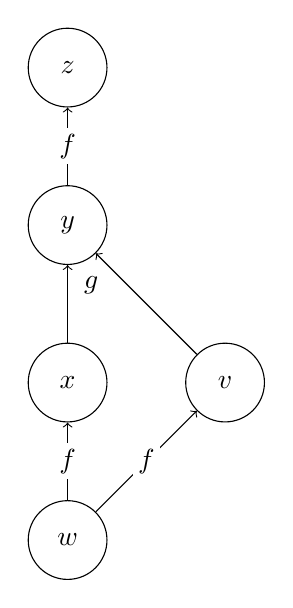
\begin{tikzpicture}
        \def\vert{2}
        \def\hori{2}
        \tikzstyle{place}=[circle, draw=black, minimum size=10mm]
        \tikzstyle{lbl}=[inner sep=2pt, fill=white]
        
        % Nodes
        \node[place] (w) at (0 * \hori, 0 * \vert) {\(w\)};

        \node[place] (x) at (0 * \hori, 1 * \vert) {\(x\)};
        \node[place] (v) at (1 * \hori, 1 * \vert) {\(v\)};
        
        \node[place, label={[shift={(0.3,-1.5)}]{\(g\)}}] (y) at (0 * \hori, 2 * \vert) {\(y\)};
        
        \node[place] (z) at (0 * \hori, 3 * \vert) {\(z\)};
        
        % Edges
        \draw [->] (w) to node[lbl]{\(f\)} (x);
        \draw [->] (w) to node[lbl]{\(f\)} (v);

        \draw [->] (x) to (y);
        \draw [->] (v) to (y);
        
        \draw [->] (y) to node[lbl]{\(f\)} (z);
        
    \end{tikzpicture}
    \caption{Example graph for back-propagation}
\end{figure}
This means that \(x = f(w), v = f(w), y = g(x,v), z = f(y)\).
Therefore
\begin{equation}
    z = f\Big( g \big( f(w),f(w) \big) \Big).
\end{equation}
If we now want to compute \(\frac{\partial z}{\partial w}\), we can do so by applying the chain rule of calculus recursively.
It follows that
\begin{align}
    \frac{\partial z}{\partial w} &= \frac{\partial z}{\partial y} \Bigg( \frac{\partial y}{\partial x} \frac{\partial x}{\partial w} + \frac{\partial y}{\partial v} \frac{\partial v}{\partial w} \Bigg) \label{eq:back-prop-example} \\
    &= \frac{\partial z}{\partial y} \Bigg( \frac{\partial y}{\partial x} + \frac{\partial y}{\partial v} \Bigg) \frac{\partial x}{\partial w}, \quad \text{because } \frac{\partial x}{\partial w} = \frac{\partial v}{\partial w} \\
    &= f^\prime (w) \cdot \Big( g^{(1,0)} \big( f(w), f(w) \big) + g^{(0,1)} \big( f(w), f(w) \big) \Big) \cdot f^\prime \big( f(w), f(w)\big).
\end{align}
Where \fref{eq:back-prop-example} describes, what the back-propagation algorithm would do.